\chapter{Change-point detection for concentration data}\label{chp:4}

\minitoc

\clearpage

In this Chapter, we build a change-point detection algorithm specially adapted for concentration data. We will use this algorithm in the subsequent chapter to detect homogeneous temporal periods on which spatial statistical inferences will be possible. Several elements presented in Chapter \ref{chp:3} are used to build this method:  
\begin{itemize}
\item We use a parametric change-point detection, more precisely a maximum likelihood based method as described in Section \ref{chp:3:1}. The cost function $W$ is defined as the negative log likelihood of a distribution $Q$. The choice of $Q$ is motivated by the observation of the data, we mentioned in Chapter \ref{chp:2} that the distributions of concentrations were right skewed and presented long tails. Probability laws such as the Weibull are used for illustrations.  
%see Chapter \ref{chp:5} for an illustration on pesticide concentration data modelling.   
\item We use the PELT search method presented in Section \ref{chp:3:4} to obtain optimal solution to the change-point detection problem. Several penalty values $\beta$ are explored with the CROPS algorithm presented in Section \ref{chp:3:4}. The elbow method is applied when it is necessary to estimate an optimal number of change-points.   
\end{itemize}
We first describe the model integrating the censoring information in Section \ref{chp:4:1}. However, we do not know how much the censoring can affect a parametric change-point model. We provide a study of censoring effects in Section \ref{chp:4:2}. Furthermore, we need to devise an estimation procedure that is adapted to the observations of pesticide concentrations. We propose an original change-point detection method, involving an iterative procedure to estimate both piecewise constant parameters and parameters constant over time in the model.
We devise our estimation scheme in Section \ref{chp:4:3}. Finally, in Section \ref{chp:4:4}, we compare our method against the \textit{Multrank} non-parametric change-point method that can take into account the censoring in the data in its cost function \citep{lung2015}. This method was reviewed in Chapter \ref{chp:3}. 

%The question sums up to detecting breaks in all dimensions of the parameters of $Q$ or not. 
\section{Generic model for censored data}\label{chp:4:1}

\subsection{Framework}

We present here the underlying parametric model which summarizes the standard model introduced in Section \ref{chp:3:1}. We consider $\bm c = c_1,\dots,c_n$ which are realizations of independent real random variables $C_1,\dots,C_n$. The variables $C_i$ are recorded sequentially, and the recording times are not necessarily equidistant. Thus, the indices in $C_i$ are only indicators of the order of occurrence in the sample and not of the observation times. We suppose that there exist $K^*$ changes in the distribution of $\bm c$ happening at indices $0=\tau_0^*<\tau^*_1 <... < \tau^*_k <... < \tau^*_{K^*}<\tau^*_{K^*+1}=n$. Moreover, on the k-th segment, all random variables in the segment $C_{\tau^*_{k-1}+1:\tau^*_{k}}$ follow a distribution $Q$ with parameters defined by the vector $\theta^*_k\in\Theta$ with $\Theta\subset\mathbb{R}^P$. We denote $\bm{\theta^*} = (\theta^*_k)_{k=0}^{K^*}$. More formally, we have that:  
$$c_t \sim \sum_{k=0}^{K^*} f(.\vert\theta^*_k)\mathbbm{1}_{\tau^*_{k}+1\leq t \leq \tau^*_{k+1}},$$
$f$ being the density function of distribution $Q$ with respect to the Lebesgue measure on $\mathbb{R}$.  


The observations are subject to censoring. We focus on left-censoring because it is adapted for modelling concentration data but similar models can be created for right censoring or a mix of both. To each $c_i$ is associated a known censoring threshold $a_i \ge 0$. The resulting censored observations are defined by:  
\begin{equation}\label{chp:4:defy}
Y_i = \sup(C_i,a_i)
\end{equation}
Since the $C_i$ are independent and the $a_i$ are known deterministic values, the $Y_i$ are independent as well. The observations of $Y_i$ are denoted $y_i$. In this model, we can write the log-likelihood of a segment $y_{\tau^*_k+1:\tau^*_{k+1}}$ as:  
\begin{equation}\label{chp:4:loglik}
\mathcal{L}(y_{\tau^*_k+1:\tau^*_{k+1}},\theta^*_k) = \sum_{i = \tau^*_k+1}^{\tau^*_{k+1}}\log(f_{\theta^*_k}(y_i)) = \sum_{i = \tau^*_k+1}^{\tau^*_{k+1}}\log(F(y_i\vert\theta^*_k))\mathbbm{1}_{y_i=a_i}+\sum_{i = \tau^*_k+1}^{\tau^*_{k+1}}\log(f(y_i \vert\theta^*_k))\mathbbm{1}_{y_i>a_i},
\end{equation}
with $f_{\theta^*_k}$ being the density function of $C_i$ for $i \in [\tau^*_k+1,\tau^*_{k+1}]$, $F(\vert\theta^*_k)$ being the cumulative distribution function (cdf) of $Q$. 

Note that if one needs to integrate right censoring into the likelihood, one should simply replace the $\sup$ in the definition \ref{chp:4:defy} by the $\inf$ of both quantities and cdf function $F$ by the survival function $S(t)=1-F(t)$. 

In practice, the values $a_i$ correspond to the values of LOQ\footnote{Limits of quantification (see Chapter \ref{chp:2:3})}. We could develop a double-censored model using both the LOD\footnote{Limits of detection (see Chapter \ref{chp:2:3})} and LOQ values. However, since the information from LOD is rarely available, we only use the LOQ.

\subsection{Estimator choices and properties}

In this section, we define the criterion to minimise and we choose the estimators of the parameters in our model. 

%We can define the cost function of a segment $y_{u:v}$ as:    
The cost function used to evaluate segments is the negative log-likelihood calculated using the maximum likelihood estimator $\widehat{\theta}_{u:v}$ of segment $y_{u:v}$: 
\begin{equation}\label{chp:4:costfunc}
W(y_{u:v}) = -\sup_{\theta\in\Theta}\{\sum_{i=u}^v\log(F(y_i,\theta))\mathbbm{1}_{y_i=a_i}+\sum_{i=u}^v\log(f(y_i,\theta))\mathbbm{1}_{y_i>a_i}\},
\end{equation}
with $F$ the cumulative distribution function (cdf) of $Q$.

Since we do not know the number of change point before hand, we opt for the penalized criterion defined in \ref{chp:3:4}. For a segmentation $\TT = \{\tau_1,...,\tau_K\}$ of a given signal $\bm y =\{y_1,\dots,y_n\}$, the penalised cost is given by: 
\begin{equation}\label{chp:4:pencost}
\CC(\bm y,\TT)=\sum_{i=0}^{K}  W(y_{\tau_i+1:\tau_{i+1}}) + KP\beta,
\end{equation}
where $P$ is the dimension of the parameters vector in the distribution $Q$ and $\beta > 0$ the penalty weight value. Gathering \eqref{chp:4:costfunc} and \eqref{chp:4:pencost}, this resulting estimator can be expressed as:  
\begin{equation}\label{chp:4:estim}
(\widehat{K},\widehat{\TT},\widehat{\bm \theta}) = \arg\min_{\TT,\bm \theta,K} \left(- \sum_{i=0}^{\lvert \TT \rvert}  \left\{\sum_{j=\tau_i+1}^{\tau_{i+1}}\log(F(y_j,\theta))\mathbbm{1}_{y_j=a_j}+\sum_{j=\tau_i+1}^{\tau_{i+1}}\log(f(y_j,\theta))\mathbbm{1}_{y_j>a_j}\right\}+\beta KP\right)
\end{equation}

%We proceed to the estimation of its parameter using the maximum likelihood estimator $\widehat{\theta}_{u:v}$ on each segment $y_{u:v}$. It is defined by:
%\begin{equation}\label{chp:4:emv}
%\widehat{\theta}_{u:v} = \arg\max_{\theta \in \Theta}\mathcal{L}(y_{u:v},\theta)
%\end{equation}

Furthermore, we assume the following on the model:  
\begin{itemize}
\item[\textbf{H1:}] $\Theta$ is compact and there exists $\Delta_{\bm \theta}^{\star}>0$ such that $\vert \theta_{k+1}^{\star}-\theta_{k}^{\star}\vert > \Delta_{\bm \theta}^{\star}$, for all $k=0,...,K^{\star}$.
\item[\textbf{H2:}] There exists $\Delta_{\bm \tau}^*>0$ such that $\vert \tau_{k}^{\star}-\tau_{k-1}^{\star}\vert > \Delta^*_{\bm \tau}$, for all $k=1,...,K^{\star}$.
\item[\textbf{H3:}]  There exists a positive integer $K_{max}$ such that the maximum number of segments $\frac{n}{\Delta^*_{\bm \tau}}$ satisfies $K_{\max} \geq \frac{n}{\Delta^*_{\bm \tau}}$. 
\item[\textbf{H4:}] The penalty value is dependant of $n$. It can be written $\beta_{n}$ and verifies $\beta_{n}\xrightarrow[n\rightarrow \infty]{} \infty$ and $\frac{\beta_{n}}{n}\xrightarrow[n\rightarrow \infty]{} 0$.
\end{itemize}

These are standard hypotheses for change point detection that can be found in \cite{Lavielle1997} or \cite{He2010}. Hypothesis \textbf{H1} mainly aims at ensuring sufficient conditions for the identifiability of the model, by imposing a minimum gap between two consecutive $\theta$'s. 

Hypothesis \textbf{H2} checks that each segment contains sufficient data for obtaining reliable estimates for the $\theta$'s and Hypothesis \textbf{H3} states the number of regimes is bounded from above.  

Hypothesis \textbf{H4} is verified by a large range of penalties including the BIC \citep{YAO1988181}. 

We formulate an additional hypothesis \textbf{H5}, which is also the strongest one. 
\begin{itemize}
\item[\textbf{H5:}] Change-point locations are independent of the scale and frequency at which the data is sampled
\end{itemize}
This hypothesis will also allow us to derive the asymptotic behaviour of the estimator, when the sample size is sufficiently large. One should note here that a larger sample means a finer scale for sampling the data and not an extension of the period of observation. 

Note that in practice, for environmental data with scarce and irregular sampling, this hypothesis is hard to verify.
However, we may suppose that the change-points occurring in concentration data are linked with the farming activities and the phyto-pharmaceutical uses, regardless of the sampling rate. 

Under these assumptions, we know that the maximum likelihood estimator computed in Equation \eqref{chp:4:estim} is weakly consistent \citep{Lavielle1997}. \begin{equation}
(\widehat{K},\widehat{\mathcal{T}},\widehat{\theta}) \xrightarrow[n\to+\infty]{\mathbb{P}} (K^*,\mathcal{T}^*,\theta^*)
\end{equation}
Elements of proof are provided in Appendix \ref{app:chap4:1}. 

%However, even when \textbf{H1} holds, censoring may cause identifiability issues that will be handled in Section \ref{chp:4:2}.
%we show in Section  that censorship could cause additional identifiability problems that will require specific .  
%implies that . 
%The sampling quality (size and regularity of   being one of the main problem of the data we are working with, it would be hard to verify asymptotic properties. 

\subsection{Estimation procedure}

\subsubsection{Estimation of parameters for a single homogeneous segment}

For a given $y_{u:v}$, one should be able to properly compute $\widehat{\theta}_{u:v}$. as the estimate of the parameter of $Q$. It is impossible to obtain a explicit formula of $\widehat{\theta}_{u:v}$ when there are censored observations in the sample. Therefore one needs to use a numerical optimisation procedure to compute the estimate. In this thesis, the Newton-Raphson method was used to search for the zeros of the first derivative of the cost function \eqref{chp:4:costfunc}.  

For some choices of $Q$, checking that the cost function is strictly convex is not always easy. However, we can still show that the cost is locally convex and has a unique minimum by studying its variations. This implies a careful choice in the parameter initialization value of the Newton-Raphson method to obtain convergence of the solution $\widehat{\theta}_{u:v}$. Appendix \ref{app:chap4:2} provides experiments on the initialization of the Newton-Raphson method. 

\subsubsection{Estimation procedure for $K^*$, $\mathcal{T}^*$ and $\theta^*$}

The estimation procedure aims at maximising the penalised log-likelihood in Equation \eqref{chp:4:pencost}. The optimisation procedure implies finding both the best partitioning of the data as defined by $\widehat{K}$ and $\widehat{\mathcal{T}}$, as well as the estimates for the parameters of the distribution $Q$ within each segment, $\widehat{\theta}$. 

We proceed using the PELT algorithm (see Section \ref{chp:3:4}). In practice, we use the following value for the cost function to evaluate a given segment $y_{u:v}$:
\begin{equation}
W(y_{u:v},\widehat{\theta}_{u:v}) = \sum_{i=u}^v\log(F(y_i,\widehat{\theta}_{u:v}))\mathbbm{1}_{y_i=a_i}+\sum_{i=u}^v\log(f(y_i,\widehat{\theta}_{u:v}))\mathbbm{1}_{y_i>a_i},
\end{equation} 
where $\widehat{\theta}_{u:v}$ is the MLE, computed numerically with the Newton-Raphson method on the segment $y_{u:v}$.
%the output of the Newton-Raphson method, trained on segment $y_{u:v}$. 

\subsubsection{Selecting the optimal number of changes}

We use the CROPS algorithm (see Section \ref{chp:3:4}) to select the optimal number of change points in the signal. The penalty range selected investigated is derived from the BIC criterion formula \citep{YAO1988181}.  
Note that this choice verifies assumption \textbf{H4}. In change point detection, the BIC penalty can be written as: 
\begin{equation}
\beta_{BIC} = \frac{P\log(n)}{2},
\end{equation}
with $P$ the dimension of the parameter $\theta$ and $n$ the length of signal $\bm y$. The range of penalty values explored in this thesis writes under the form: 
\begin{equation}
[\beta_{min},\beta_{max}] = \left[\frac{\beta_{BIC}}{j},\beta_{BIC}\times m\right],
\end{equation}
with $j,m\in\mathbb{N}$. Hence, our penalty range is calibrated accordingly to Hypothesis \textbf{H4} because $\beta_{min}$ and $\beta_{max}$ also verify its conditions.  

We choose the value of $j$ such that the penalty $\frac{\beta_{BIC}}{j}$ is associated to what would seem to be an overfitting segmentation model. More precisely, we look for $j$ such that associated number of change points is close to the maximal number of segments possible given the minimal segment size chosen in PELT. 

Likewise, $m$ is chosen such that the penalty $\beta_{BIC}\times m$ is associated to an underfitting segmentation model. More precisely, we look for $m$ such that associated number of change points is close to zero.     

Once we run CROPS, we obtain some penalty values $\{\beta_{min},\dots,\beta_{max}\}$. Since each of these penalty values is associated to a segmentation cost and a number of change points, we can perform the elbow method heuristic (see Algorithm \ref{chp:3:algoelbow}) on the curve of the segmentation costs plotted against the number of changes. An optimal number of break points and the associated segmentation are thus selected with this procedure.
%Let us mention here that Algorithm 1 relies on a series of hyper-parameters which ought to be tuned: the precision threshold and the maximum number of iterations in the Newton-Raphson step, the initial values for the l’s in Newton-Raphson step also, and the minimum number of observations between two consecutive change-points. In the experiments we performed, the initial values for the l’s were set as the inverse of the observed average value in the respective segment.
%the thus guaranteeing the unicity of the maximum likelihood estimate.
%\rightarrow_{n\to+\infty}^{\mathbb{P}}
%Although these hypotheses guarantee the convergence of estimates in the classical framework (e.g. just as in \cite{Lavielle1997}), we need to examine the effects of censoring in our method, which is a factor that places us out of the classical framework.

Let us now study the effect of censoring on our procedure.

\section{Censoring effects}\label{chp:4:2}

%We are interested in the effects of censorship on two main aspects: 
%\begin{itemize}
%\item The quality of the estimation of the parameters $\bm \theta$ of $Q$ on a fixed segment. 
%\item The implication it can have on the search method PELT and how to adapt it if this is the case. 
%\end{itemize} 
%
%\subsection{On the parameter estimation for one segment}\label{chp:4:cens_seg}
%On the change point detection method

The censoring can be an issue in the practical implementation of the procedure developed in Section \ref{chp:4:1}. In particular, issues can be encountered when estimating the parameter of a fully censored segment with Newton-Raphson. Illustrating examples are provided in this section with $Q$ set as the exponential distribution.

\subsection{Practical problem encountered with censoring}\label{chp:4:cens_seg}

%The cost functions need to be twice differentiable in $\theta$. We search for the zeros of the first derivative of the cost function in order to find a global minimum. 
%Checking that the second derivative is strictly positive in presence of censored data, thus guaranteeing the unicity of the maximum likelihood estimate, can prove to be a difficult task as it is not always the case for all distributions $Q$. 
%We provide an example of such a case in Appendix \ref{app:chap4:2} where we prove the existence of a global minimum without having the global convexity of the first derivate. 
%Looking at the analytical likelihood formula, we find that the $\theta$ realising the minimum of the cost function is still unique, but tends toward infinity. 

In general, an explicit formula for the maximum likelihood estimator (MLE) is not available in presence of censored data, leading to the use of numerical methods for its computation. The Newton-Raphson method was used on each segment to compute the MLE estimate of $\theta$. 

Specifically, the case where all data in the segment $y_{u:v}$ are censored is problematic. The estimation of $\theta$ is impossible. We illustrate in Figure \ref{fig:onlycens} with $Q$ set as an exponential distribution of parameter $\theta = \lambda$. 
For a given segment $y_{u:v}$ where all observations are censored and under a censoring threshold $a$ we have that: 
\begin{equation} \label{chp:4:costex}
W(y_{u:v}) = -\sup_{\lambda \in ]0;+\infty[}(v-u)\log(1-\exp(-\lambda a)) 
\end{equation}
This cost is always positive and decreasing to 0 when $\lambda$ goes to infinity. 
\begin{figure}[ht]
    \centering
    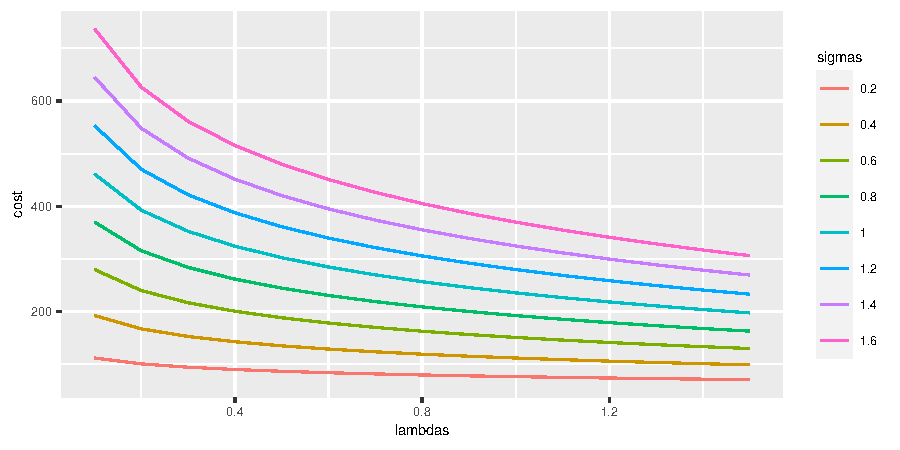
\includegraphics{figs/Chap4/only_cens.pdf}
    \caption{Plot of the cost function values against $\theta$ values when all observations are censored. It is represented for an exponential distribution. The sample consists in 100 values of censored observations to a threshold $a = 0.05$.}
    \label{fig:onlycens}
\end{figure}
%We show in the next part why it could be problematic to have fully censored segments in the search method and how we chose to deal with it. 
%\subsection{On the change point detection method}

We made the assumption that the support $\Theta$ of the segments parameters is a compact of $\mathbb{R}^P$ in Section \ref{chp:4:1} . This corresponds to hypothesis \textbf{H1}. Hence, we need to decide of an upper bound for $\theta$. We show in the next section how we proceed. 

%This means that there is an upper bound $\theta_{max}$ such that $\theta\geq\theta_{max}$ for all $\theta$.
%The case of fully censored segments are questioning the identifiability of the change-point detection method. This assumption is summarized in hypothesis \textbf{H1} of Section \ref{chp:4:1}.  
%\citep{Lavielle1997} 
%for the segment parameters is the following:   
%\begin{itemize}
%\item[] $\Theta$ is compact and there exists $\Delta_{\bm \theta}^{\star}>0$ such that $\vert \theta_{k+1}^{\star}-\theta_{k}^{\star}\vert > \Delta_{\bm \theta}^{\star}$, for all $k=0,...,K^{\star}$. 
%\end{itemize}

\subsection{Introduction of an upper bound parameter on $\theta$}

%If that is the case $\Theta$ is not compact.
We have seen in Section \ref{chp:4:cens_seg} that, for the exponential distribution example, the optimal $\theta$ tends to infinity. To solve this practical problem, we introduce an additional parameter $\theta_{max}$ in our implementation such that $\theta$ is constrained to the interval $[0,\theta_{max}]$ which is a compact part of $\mathbbm{R}$. 

A new problem arises from this modelling choice. The value of $\theta_{max}$ must be chosen carefully. We must ensure that $\theta_{max}> \theta^*_k,$ for all $k \in \{0,\dots,K^*\}$. If it is not the case, the identifiability problem remains. For two $\theta^*_i$ and $\theta^*_j$  greater than $\theta_{max}$, their estimates will be set to $\theta_{max}$ and thus no segment identifiability will be possible. 

In order to avoid such problems, the value of $\theta_{max}$ is set according to the worst possible censoring case. More precisely, we assume that no change-point occurred in $\bm y$ and that all observations are distributed according to $Q$ with parameter $\theta_{max}$. We set $\theta_{max}$ to the value such that: 
\begin{equation}\label{chp:4:thetamax}
F(\min(\bm y),\theta_{max})^n = \alpha,
\end{equation}
with $\alpha$ being a desired percentage of censoring. In practice, we decide to set $\alpha$ to $95\%$. This corresponds to the scenario where there is a $95\%$ chance that $n$ observations generated from the distribution $Q$ with parameter $\theta_{max}$ are left-censored and under the threshold $a = \min(\bm y)$. \\
% $95\%$ of the observation in $\bm y$ would be censored and would be less to the smallest censoring threshold value. 

We provide a practical example with the exponential distribution. We simulate a signal $\bm y$ of size $n = 200$ that is a realization of exponential distributions of parameters $\lambda^*_0 = 1$ for $y_{1:100}$ and $\lambda^*_1 = 4$ for $y_{101:200}$. The censoring level is set to the median of $\bm y$ so that 50$\%$ of the signal is censored. We illustrate $\bm y$ in Figure \ref{fig:theta_max}. We choose $\lambda_{max}$ by setting $\alpha$ to $95\%$. We have that $\lambda_{max} = \frac{-\log(1-\alpha^{1/n})}{\min(\bm y)}$. In our numerical example, $\lambda_{max} = 24.68$, which is greater than $\lambda_0$ and $\lambda_1$. \\

\begin{figure}[ht]
    \centering
    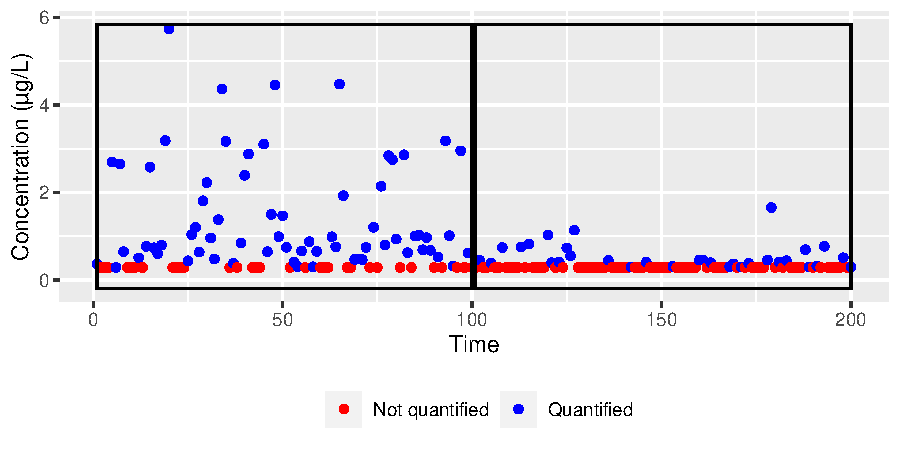
\includegraphics{figs/Chap4/theta_max_ex.pdf}
    \caption{Simulated signal $\bm y$ with distribution $Q$ set as the exponential law. \\
    The two segments are drawn with black rectangles. $\theta^*_0 = 1$ in the left segment, $\theta^*_1 = 4$ in the right one and the censoring threshold $a = 0.28$ in both segments.}
    \label{fig:theta_max}
\end{figure}

Note that other ways to tackle fully censored segments are possible. The modification of the pruning rule \eqref{chp:3:pruning} used in PELT can also be investigated. For example, one could decide to systematically discard all potential change-point indices $\tau \in \{u,\dots,v\}$ when evaluating a fully censored segment $y_{u:v}$.  

\section{Estimation with non-additive cost function: mixing fixed and changing parameter estimation}\label{chp:4:3}

%When $\theta$ is a parameter vector of dimension $P>1$, a common strategy is to opt for simultaneous changes detection in all $P$ parameters simultaneously. This implies detecting changes in different properties of $\bm y$. In practice, it depends on what parameters are optimized in the cost function. The optimization can still be performed with numerical methods (such as Newton-Raphson) on all dimensions of $\theta$ simultaneously. Plugging an estimator of the parameters vector in a cost function defined in Equation \ref{chp:4:costfunc} would results in
%Using a MLE estimators of all $P$ parameters as the supremum in \ref{chp:4:costfunc} provide a cost function that detects changes occurring in any of the parameters.  
%We can distinguish 
%In the first case,  the detection is made in all dimension of the parameter vector. In this case, this implies detecting changes in different characteristics of $\bm y$ simultaneously (for example mean and variance). 


Two different cases can occur when the parameter $\theta$ is a vector of dimension $P > 1$.  

%for a Gaussian distribution. 
In the first case, we assume that all components of the parameter $\theta$ are subject to change. This is the usual framework for change point detection as presented in Chapter \ref{chp:3} and Sections \ref{chp:4:1} and \ref{chp:4:2}. This means that changes in different parameters of $\bm y$, such as the mean and variance, are detected simultaneously. In practice with censored data, it is still possible to calculate the maximum likelihood estimator of a segment using numerical methods (such as Newton-Raphson). The problem with such a modelling choice is the number of data needed in a segment to estimate all parameters. If the number of parameters to be estimated is high, the number of observations must be more important to obtain a valid statistical estimate. 


In the second case, it is assumed that some dimensions of the parameter vector $\theta$ are constant over time. In this case, three scenarios are possible: 
\begin{itemize}
\item The fixed parameters are known. This framework is then equivalent to the first case presented above. We can estimate the parameters that are changing using what is presented in Chapter \ref{chp:3} and Sections \ref{chp:4:1} and \ref{chp:4:2}. 
\item The fixed parameters are unknown and we do not want to estimate them. In this case, the estimation of the changing parameters can be done with an appropriate cost function. For example, a quadratic loss function is practical for detecting changes in the mean of a signal without estimating the variance (which is assumed to be fixed) \citep{Fearnhead2018a}.
\item  The fixed parameters are unknown and we want to estimate them.
\end{itemize}

We are interested in the latter scenario. In the context of environmental data, the assumption that some dimensions of $\theta$ are fixed may indeed be justified if some parameter values are supposed to control the intrinsic diffusion properties of a chemical substance in the environment. Then these parameters should be invariant in time. The parameters specific to each segment could, for example, represent different intensities in the use of the substance in time. 

Note that in this framework, all estimation schemes using PELT or other dynamic programming methods are not valid. These methods rely on the fact that the criterion to be optimised is additive, which is no longer the case. There are other methods for estimating signal changes that do not require this property, such as MCMC algorithms \citep{Lavielle2001} or genetic algorithms, but they are outside the scope of this thesis. 

This section develop our own estimation strategy.

%we can either suppose that the fixed parameters are known in which case the change point detection procedure can be done with an appropriate cost function. For example a quadratic loss function is practical for detecting changes in the mean of a signal without estimating the variance (that is supposed to be fixed) \citep{Fearnhead2018a}. 
%this modelling choice

%An example with $Q$ set as a Weibull distribution is provided in Figure \ref{fig:param_ex}. 
%\begin{figure}[ht]
%    \centering
%    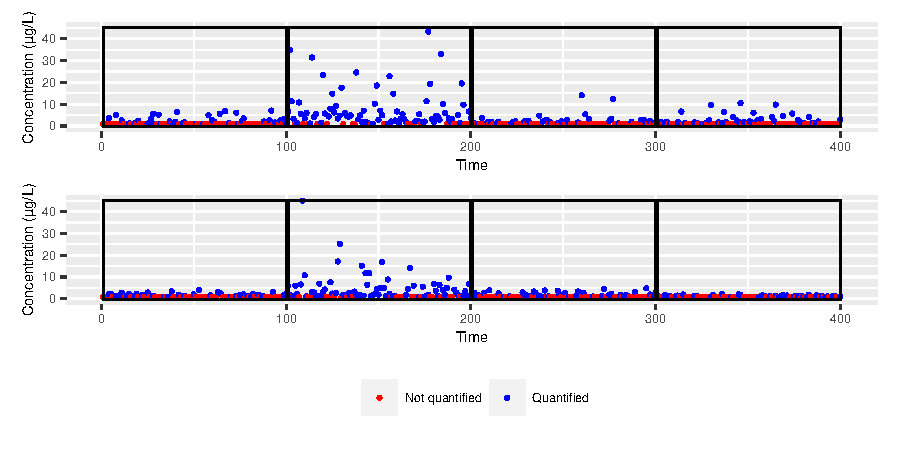
\includegraphics{figs/Chap4/param_ex.pdf}
%    \caption{Example of simulated signal $\bm y$ distributed according Weibull distributions with $(\lambda,\sigma)$ as the scale and shape parameters. The segments are drawn with black rectangles. \\ 
%\textbf{Upper signal:} The associated parameters to each segment are $\theta^*_{0,.} = (\lambda^*_0,\sigma^*_0) = (1,1)$, $\theta^*_{1,.} = (\lambda^*_1,\sigma^*_1) = (3,0.7)$, $\theta^*_{2,.} = (\lambda^*_2,\sigma^*_2) = (1,0.7)$, $\theta^*_{3,.} = (\lambda^*_3,\sigma^*_3) = (1,2)$ and the censoring threshold $a = 0.86$ in all segments.\\
%\textbf{Lower signal:} The associated parameters to each segment are $\theta^*_{0,.} = (\lambda^*_0,\sigma^*) = (1,0.7)$, $\theta^*_{1,.} = (\lambda^*_1,\sigma^*) = (5,0.7)$, $\theta^*_{2,.} = (\lambda^*_2,\sigma^*) = (0.7,0.7)$, $\theta^*_{3,.} = (\lambda^*_3,\sigma^*) = (1,0.7)$ and the censoring threshold $a = 0.89$ in all segments.}
%    \label{fig:param_ex}
%\end{figure}

\subsection{Estimators of a segmentation with some fixed parameters}
%the parameter estimation proposed in

%We discuss here the procedure for solving the parameter estimation problem \eqref{chp:4:estim}. When $\theta^* \in \mathbb{R}^P$ with $P > 1$, several optimization strategies are possible. 
We use the following notations in this section: 
\begin{itemize}
\item $\bm \theta_{.,m} = (\theta_{0,m},\dots,\theta_{K,m})$ is the m-th dimension of the parameter vector of each segment $k$.
\item $\bm \theta_{k,.} = (\theta_{k,1},\dots,\theta_{k,P})$ is the parameter vector of the k-th segment.
\item $\theta_{k,m}$ is the m-th dimension of the parameter vector of the k-th segment.
\end{itemize}

We are interested in models where changes occur only in some dimensions of $\bm\theta^*$. We denote $\mathcal{M} \subset \{1,\dots,P\}$ the set of indices of dimensions where the changes occur and $\overline{\mathcal{M}}$ the complementary set. We introduce the notations $(\bm\theta^*_{.,m})_{m \in \mathcal{M}} := \bm\theta^*_{\mathcal{M}}$ and $(\bm\theta^*_{.,m})_{m \in \overline{\mathcal{M}}} := \bm\theta^*_{\overline{\mathcal{M}}}$

 Therefore, the parameters $\bm\theta^*_{\overline{\mathcal{M}}}$ are reduced to a vector of fixed parameters throughout the signal $\bm y$. In this setting, the estimation procedure differs from Equation \eqref{chp:4:estim} and can be expressed as: 

    %Figure \ref{fig:param_ex} provides an illustration of signal $\bm y$ simulated with these assumptions. 

\begin{dmath}\label{chp:4:estimproc}
(\widehat{K},\widehat{\TT},\widehat{\theta}_{\mathcal{M}},\widehat{\theta}_{\overline{\mathcal{M}}}) = \arg\min_{K,\TT,\bm \theta_{\mathcal{M}},\theta_{\overline{\mathcal{M}}}}\bigg[\bigg\{ - \sum_{i=0}^{\lvert \TT \rvert}  \left(\sum_{j=\tau_i+1}^{\tau_{i+1}}\log(F(y_j,\theta))\mathbbm{1}_{y_j=a_j}+\sum_{j=\tau_i+1}^{\tau_{i+1}}\log(f(y_j,\theta))\mathbbm{1}_{y_j>a_j}\right)\bigg\}+\beta KP \bigg]
\end{dmath}

Unfortunately the criterion in Equation \eqref{chp:4:estimproc} is not additive as constant parameters introduce dependencies between the costs of each time segment. We cannot leverage the additivity property to obtain fast algorithms based on dynamic programming. We propose therefore to use an alternating optimisation procedure described in the following section. 

From Equation \eqref{chp:4:estimproc}, we can now design a two-step iterative estimation strategy.


\subsection{Estimation procedure}\label{chp:4:3:2}

%The two steps of each iteration can be described as:

We describe the practical implementation of the estimators defined in Equation \eqref{chp:4:estimproc}. We choose to proceed with two nested steps: the inner step uses an alternating optimization scheme to solve problem \eqref{chp:4:estimproc} for a fixed value of $\beta$ while the outer step explores a range of values for $\beta$.

\subsubsection{Inner step}\label{chp:4:3:2:1}

For a fixed penalty value $\beta$ in a range $[\beta_{min},\beta_{max}]$ and an initial $\widehat{\bm\theta}_{\overline{\mathcal{M}}}$, we iterate the following two steps until convergence: 
\begin{enumerate}
\item Run the PELT algorithm with penalty $\beta$ and fixed $\widehat{\bm\theta}_{{\overline{\mathcal{M}}}}$ to estimate $\widehat{\TT}$ and $\widehat{\bm\theta}_{\mathcal{M}}$.
\item Compute the MLE $\widehat{\bm\theta}_{{\overline{\mathcal{M}}}}$ with fixed $\widehat{\TT}$ and $\widehat{\bm\theta}_{\mathcal{M}}$ with any optimization method that handles censored data. We use the \texttt{R} package developed in \cite{delignette2015} in our procedure.  
\end{enumerate} 

The initialization is an important part of this procedure. We would like the initial estimate of the fixed parameters to be close to $\bm\theta^*_{{\overline{\mathcal{M}}}}$ to ensure the convergence of the procedure. In order to do so, we initialise $\widehat{\bm\theta}_{\overline{\mathcal{M}}}$ assuming no change-point occurred in $\bm y$.  More precisely, in this case $\bm\theta^*$ is a vector and we use the MLE estimator:  
\begin{equation}\label{chp:4:init}
\widehat{\bm\theta} = \arg\min_{\theta}\bigg\{ - \left(\sum_{j=1}^{n}\log(F(y_j,\theta))\mathbbm{1}_{y_j=a_j}+\sum_{j=1}^{n}\log(f(y_j,\theta))\mathbbm{1}_{y_j>a_j}\right)\bigg\},
\end{equation}   
which implies using iterative methods again as stated in \cite{cohen1965maximum}.

The initial value of the vector $\widehat{\bm\theta}_{\overline{\mathcal{M}}}$ is initialized with the corresponding coordinates in $\widehat{\bm\theta}$. Note that the initialization does not depend on the penalty value $\beta$. 
%We choose the initial values as the  such that $m\in$. 
%It can be noted straight away that the value of $\widehat{\bm\theta}_{.,m\in\mathcal{M}}$ will be discarded since it was computed from a model that goes in direct contradiction with the assumption in \ref{chp:4:1} that they were change-points in the signal $\bm y$. 

%In the second step of an iteration, we compute a new segmentation from the value of $\widehat{\bm\theta}_{{.,m\in\overline{\mathcal{M}}}}$ using a similar procedure as the one described in Section \ref{chp:4:1}. More precisely, we run PELT several times on penalty values included in a range $[\beta_{min},\beta_{max]}$. Once several results of segmentation are acquired, $\widehat{\TT}$ and $\widehat{\theta}_{.,m\in\mathcal{M}}$ are chosen using the elbow heuristic as proposed in Section \ref{chp:3:3}.   

\subsubsection{Outer step}\label{chp:4:3:2:2}

This step aims at selecting penalty values $\beta$ in a given range $[\beta_{min},\beta_{max}]$.

A first simple approach is to define an evenly spaced penalty grid $(\beta_{min},\dots,\beta_q,\dots,\beta_{max})$ where $\beta_{min}<\dots<\beta_{q}<\dots<\beta_{max}$. The inner step is performed on each of these $\beta_{q}$. Eventually, the optimal penalty value, hence the corresponding parameters, is selected using an elbow rule heuristic as proposed in Section \ref{chp:3:3}.

Another option is to use the CROPS algorithm to explore the penalty range since this algorithm only requires the penalty term to be linear and number of breaks to be non increasing with respect to the penalty weight, without any other specific assumption on the cost function. In particular, it does not require the cost function to be additive. 
\newline
\newline

%We show the relevance of the PELT step in the inner loop of this estimation procedure in Appendix \ref{app:chap4:3}. 
We verify in Appendix \ref{app:chap4:3} that the theoretical conditions needed for PELT to provide an optimal solution are fulfilled in the inner step. The next section is devoted to the evaluation of the efficiency of our method through numerical simulations. This optimisation method will be used later in Chapter \ref{chp:5}.


%We show the efficiency of this nest estimation procedure in Appendix \ref{app:chap4:3}, it will be used in Chapter \ref{chp:5}. We compare the efficiency of our method against a state-of-the-art in the next section.

%The difference is that we do not use the CROPS algorithm to explore the penalty range. Instead, we use a penalty grid  are evenly spaced. 
%This can be justified by the fact that the penalty values explored by CROPS would change at each iteration. We want to be sure that the selection step made with the elbow heuristic is made on segmentations issued from the same penalty values. 
%we want to be able to compare each set of segmentations at each iteration. Since ,  

%the estimated segmentation $\widehat{\TT}$ and the fitted parameters on its segments $\widehat{\theta}_{.,m\in\mathcal{M}}$ are obtained by applying the PELT procedure \citep{Killick2012}. PELT is run several times on a penalty grid $(\beta_0,\dots,\beta_q,\dots,\beta_{B})$ where $\beta_0<\dots<\beta_{q}<\dots<\beta_{B}$ are evenly spaced. We obtain $B$ segmentations of $\bm{y}$. 

\section{Simulation study}\label{chp:4:4}

%We test our method on simulated data and compare it with the \textit{Multrank} method \citep{lung2015}. This section aims at two objectives. First, we want to calibrate the parameters in the PELT search method to ensure a good detection capacity. Then, we want to test if that calibration really leads to better change-point results.  

In this section we conduct experiments with simulated data. For all simulated data, the distribution $Q$ is set as a Weibull law with the scale parameter $\lambda$ and the shape parameter $\sigma$. The data are simulated so that $\lambda$ is the parameter whose value changes, while $\sigma$ is constant across the simulated signals.  

First, we want to calibrate the minimum segment size parameter in the PELT search method. We recall that this method is used for the segmentation step (inner step \ref{chp:4:3:2:1}) of our algorithm. We define a simple framework in these experiments by assuming that the value of $\sigma$ is known. Comparisons are made with the \textit{MultRank} non-parametric method \citep{lung2015} to establish a satisfactory value for the minimum segment size (see Section \ref{chp:4:4:1}).  

We then compare the performance of parametric change point detection with the \textit{MultRank} method once again. The $\sigma$ should also be known in this framework. This time, these experiments are performed to confirm that calibration of the minimum segment length value in \ref{chp:4:4:1} results in correct change point detection. More complex signals are simulated, e.g. signals with multiple change points (see Section \ref{chp:4:4:2}).  

Finally in section \ref{chp:4:4:3}, we discuss the results of the estimation procedure developed in Section \ref{chp:4:3:2:2}. In this case, the shape parameter $\sigma$ is unknown and must also be estimated with the positions (and the number) of the change points and the scale parameters of each segments. 
%Two outer step procedures are tested on two complex simulated signals.  

\subsection{Calibration of the minimum segment size}\label{chp:4:4:1}


%The test based on the LR statistic consists in comparing $\Lambda$ with a threshold $B$. If $\Lambda \geq B$, we assume that $\mathcal{H}_1$ is correct. Note that if $\Lambda \geq B$, we can write:
%\begin{align}
%\Lambda &\geq B 
%\iff \sum_{i=1}^n\log(f(y_i\vert\theta_0))-\sum_{i=1}^t\log(f(y_i\vert\theta_1))-\sum_{i=t+1}^n\log(f(y_i\vert\theta_2)) &geq \log(B) \\
%\iff \sum_{i=1}^n\log(f(y_i\vert\theta_0)) &\geq \sum_{i=1}^t\log(f(y_i\vert\theta_1))+\sum_{i=t+1}^n\log(f(y_i\vert\theta_2))+\log(B) \\
%\iff 
%\end{align}
 
%We denote $W(\bm y_{1:n})$ the unpenalized cost of the optimal segmentation of $\bm y$ with $K$ change points. 
%Indeed, the likelihood ratio is constructed by calculating the likelihood of the total signal in the numerator and the likelihood of the optimal segmentation with a single break in the denominator. 

%Assessing the detection capacity of our procedure is equivalent to  since the negative log-likelihood defines the cost function in our procedure.    

In this section, we use the Weibull distribution for the distribution $Q$. The parameters of the simulated signals are:
\begin{itemize}
\item $n$ the signal size.
\item $K^*$ the number of changes in the scale parameter values.
\item $(\tau^*_k)_{k = 1}^{K^*}$ the position of these changes.
\item $(\lambda^*_k)_{k = 0}^{K^*}$ the scale parameters of each segment.
\item $\sigma^*$ the known shape parameter.
\item $\alpha$ the censoring rate of the signal.
\end{itemize}
Note that $\alpha$ is a global \textit{a posteriori} censoring level. For a given signal $\bm y$ and $\alpha$ censoring level, the resulting censoring threshold is the empirical $\alpha$-quantile of $\bm y$.   
\newline

In section \ref{chp:2:2}, the PELT Algorithm \ref{chp:3:algopelt} introduces a minimal segment length $n_{min}$. We conduct some simulation tests to calibrate this parameter. We need to identify $n_{min}$ so that the cost function defined in \eqref{chp:4:costfunc} has sufficient data to detect a change between two segments with different parameters. This can be viewed as a classification task. We want to know if our method is able to correctly classify signals that have a change point or not.  

It can be noted that the PELT detection ability and the likelihood ratio statistic (LR) are linked when dealing with a single change point. Let $\bm y$ be a signal of size $n$. The LR statistic is used to test the hypothesis::
\begin{itemize}
\item[$\mathcal{H}_0$]: there is no change point in $\bm y$ and $y_1,\dots,y_n$ was generated by the law $Q_0$.
\item[$\mathcal{H}_1$]: there exists an index $t$ such that $y_1,\dots,y_t$ was generated by the law $Q_1$ and $y_{t+1},\dots,y_{n}$ by the law $Q_2$.
\end{itemize}
Using the notations from Equation \eqref{chp:4:costfunc}, the LR statistics writes as:
\begin{equation}\label{chp:4:LR}
\Lambda = 2(W(y_{1:n})-(W(y_{1:\widehat{t}})+W(y_{\widehat{t}+1:n}))),
\end{equation} 
where $\widehat{t}$ is the estimated change point location under hypothesis $\mathcal{H}_1$. $\widehat{t}$ can be computed with the optimal partition Algorithm \ref{chp:3:algoopt}.  

%we can see that there is no change point detected if $\Lambda$ is close to 0. hypothesis
% hint at the presence of a change point in $\bm y$. 
Under $\mathcal{H}_0$, we can expect low values of $\Lambda$. On the contrary, high values of $\Lambda$ will lead to question the validity of $\mathcal{H}_0$. Looking at the inequality $\Lambda \geq B$ with $B > 0$, we can finally write that: 
 \begin{equation}\label{chp:4:rel}
 \Lambda \geq B \iff W(y_{1:n}) \geq W(y_{1:\widehat{t}})+W(y_{\widehat{t}+1:n})+\frac{B}{2}
 \end{equation} 

Equation \eqref{chp:4:rel} shows that comparing the likelihood ratio $\Lambda$ to a threshold $B$ is equivalent to comparing the penalized cost of a single change-point model for $\bm y$ with penalty value $\frac{B}{2}$ to the cost of the whole signal without change-point.

We can then achieve a diagnosis of the classification ability of the PELT method building ROC curves of likelihood ratio statistics \citep{Fawcett2006} e.g. studying the variation of false positive and true positive rates when the decision threshold $B$ varies. Summarising the ROC curve with the Area Under Curve criteria gives a general idea of the classifying performance of the likelihood ratio statistic (thus of the PELT method).

A comparison of our method is made with the \textit{MultRank} method that is based on non parametric inference that we presented in Section \ref{chp:3:1}. More precisely, this method relies on the statistic $S_n$ defined in Equation \eqref{chp2:stattestnp}. The decision in this statistical test is also made by comparing this statistic to a threshold $B$. Thus, we can also compute a ROC curve from several $S_n$ statistics.  

%We will use this comparison to calibrate our method performance. 

We want to assess the detection ability of the PELT method in function of its minimum segment size. The simulation protocol is the following:  
\begin{enumerate}
\item For a given value of $n_{min}$, we simulate $M$ signals of size $n$. $\frac{M}{2}$ signals are simulated according to hypotheses $\mathcal{H}_0$ and $\frac{M}{2}$ according to $\mathcal{H}_1$.
\item For each of these signals, we compute the LR statistic $\Lambda$ and the $S_n$ statistic of the \textit{Multrank} method. For the parametric case, we compute the optimal segmentation with a single change point using the optimal partition Algorithm \ref{chp:3:algoopt} with the minimum segment size constraint $n_{min}$. This constraint is also implemented on the calculation of the $S_n$ statistic.  
\item From the $M$ LR statistics and the $M$ $S_n$ statistics, we construct the ROC curves for both methods and we summarise it calculating its AUC. 
\end{enumerate}

We test several configurations with different values of $n_{min} = (5,10,25,50,75)$ and different censoring levels $\alpha = (5\%,25\%,50\%,75\%,95\%)$. For each configuration, we simulate $M = 1000$ signals of size $n = 200$. 

The parameters used to simulate under hypothesis $\mathcal{H}_0$ are: $\sigma = 0.5$, $\theta_0 = 1$. Under hypothesis $\mathcal{H}_1$, we set the parameters as: $\sigma = 0.5$, $\lambda^*_1 = 1$, $\lambda^*_2 = 3$, $t = 100$. 


\begin{figure}[ht]
\centering
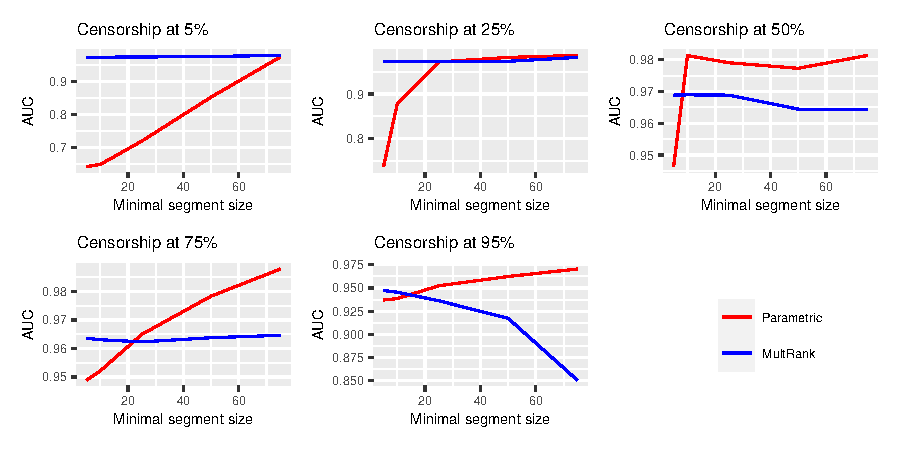
\includegraphics{figs/Chap4/sim_minseg.pdf}
\caption{Choice of the minimal segment length: simulation results. Our method performance is illustrated with the red dots, the \textit{Multrank} method is drawn in blue.}
\label{fig:sim_minseg}
\end{figure}

From the results of Figure \ref{fig:sim_minseg}, three comments can be made:  
\begin{itemize}
\item Both methods are efficient in their abilities to detect change-points in signal. The AUC are above 0.9 (except for the parametric method in a highly censored configuration with a low value minimal segment size). That make them both good classifiers. 
\item The performance of the parametric method increases with the minimum segment length. 
\item The more the censoring level increases, the more data is needed in the minimal segment length of the parametric method to outclass the non parametric method. 
\end{itemize}

We summarize our results in the two following points. Firstly, the minimum segment size depends on the censoring level. Secondly, the parametric method outperforms \textit{Multrank} for large enough minimum segment size even up to 75\% of censoring level.

It should be noted that we chose an easy simulation scenario on purpose. The parameters on each side of the change point (in the signals simulated under $\mathcal{H}_1$) do not have close values, the position of the change point is right in the middle of the signals and the data is truly distributed according to a Weibull distribution. This can explain the better classification using the likelihood ratio statistic. 

However, we can also say that if the Weibull model seems to be a good model for a real dataset, we can expect good performances on the detection ability of the parametric method. 

%, we should get the censoring level information in order to calibrate the minimal segment length of the parametric method.  
% mais si jamais avoir à faire avec données pour lesquelmes la loi de Weibull est un bon modèle on peut s'attendre de bonnes performances. 

\subsection{Testing the precision of the detection method with known $\sigma$}\label{chp:4:4:2}

We want to compare the performance of the change-point detection with the Multrank method developed in \cite{lung2015} since both methods are adapted to censored data. We examine the capacity to estimate the correct number of breaks in a signal and the precision of the change-point position. This section is illustrated using the Weibull distribution.   

The experimental framework is as follows: 
    \begin{enumerate}
        \item we simulate $M=100$ samples $(x_1,...,x_n)$ of size $n=400$  following a left-censored Weibull distribution with $\alpha\%$ of censored data. We made tests for the different censoring rates $\alpha = (25\%,50\%,75\%,95\%)$. The shape parameter of the Weibull distribution is assumed to be known and set to $\sigma=0.5$. The scaling parameters $\bm{\lambda^\star}$ have $K^\star=4$ breaks at positions $\tau^\star_1 = 80$, $\tau^\star_2 = 160$, $\tau^\star_3 = 240$ and $\tau^\star_4 = 320$ and take the values $\bm{\lambda^\star}=(\lambda^\star_1 = 1, \lambda^\star_2 = 4, \lambda^\star_3 = 0.5, \lambda^\star_4 = 5, \lambda^\star_5 = 1)$. 
        %An example of a sample simulated in this way is shown in Figure \ref{fig:ex_sim}.
        \item For each of the $M$ samples, we apply the parametric change-point detection and the Multrank methods. For each sample, we obtain the estimated number of breaks $\hat K_{param}$ and $\hat K_{multrank}$ and their position $(\hat{\tau}_{k,param})_{k = 1}^{\hat K_{param}}$ (respectively $(\hat{\tau}_{k,multrank})_{k = 1}^{\hat K_{multrank}}$). We set the minimum segment size $n_{min} =  25$. We have seen in the previous section that this is still a minimum segment size where the parametric method outperforms the \textit{MultRank} (except in highly censored signals).    
        \item For both methods, we count the number of samples among the $M$ for which the correct number of breaks has been estimated (e.g. $\hat K_{param} = K^\star$). Also, we make a histogram of the change-point positions of the samples for which $K^\star$ is estimated correctly. 
    \end{enumerate}
Since $K$ is not known, we proceed as follows for each method to estimate it:
    \begin{itemize}
        \item For the parametric method: we use the CROPS algorithm to scan a continuous range of penalty values $[\beta_{min},\beta_{max}]$. We obtain a set of $B$ values $(\hat \beta_1,...,\beta_B)$ and the optimal segmentations associated with these penalty values. We then plot the cost of the segmentations as a function of the number of breaks. We choose the optimal penalty using a elbow heuristic. This procedure is described in \cite{haynes2014}. The choice of $\beta_{min}$ and $\beta_{max}$ is inspired from linear penalties like the BIC criterion \cite{YAO1988181}. Note that when using the BIC penalty in change point detection, the penalty term written in Section \ref{chp:4:1} becomes : $\beta_n = \frac{P}{2}\log(n) = \frac{1}{2}\log(n)$, where $P$ is the number of dimensions of the parameter. More precisely, we took a wide interval of penalty values defined by $\beta_{min} = \frac{\log(n)}{10}$ and $\beta_{max} = 5\log(n)$.
        \item For the non-parametric \textit{Multrank} method, we compute the optimal segmentation using the optimal partition search method presented in Algorithm \ref{chp:3:algoopt} for $K_{max}$ change-points. For each of these segmentations, we can compute the cost of the segmentations using the cost function in \eqref{chp2:costfuncnp}. As in the parametric method, we represent the costs as a function of the number of change points, and we determine the number of estimated breaks by an elbow heuristic. Here, $K_{max}$ is fixed at $2*K^\star = 8$.
    \end{itemize}
The results of the simulations are shown in Table \ref{tab:simcomp} and in Figure \ref{fig:prec_sim}. It can be seen that in the ideal scenario, where the data are indeed distributed according to a left-censored Weibull distribution, the parametric method performs better both in detecting the correct number of breaks and in accurately estimating their position. However, this performance decreases as the censoring rate increases.

%\begin{figure}[htbp]
%    \centering
%    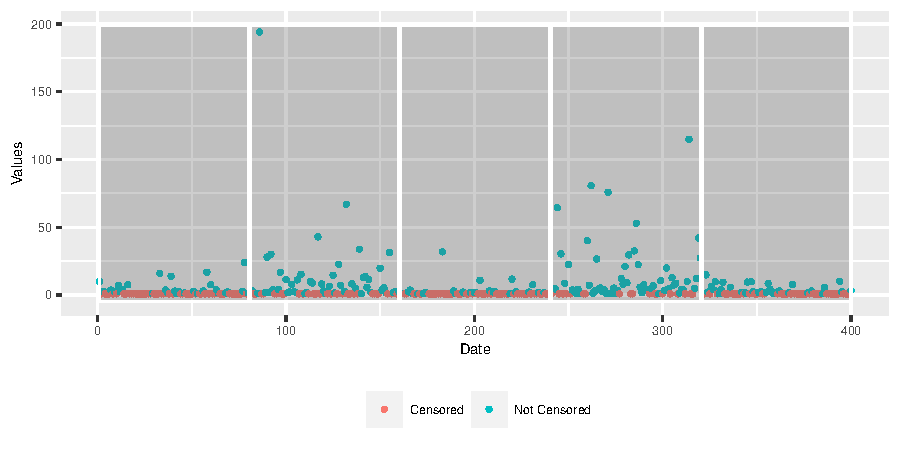
\includegraphics{figs/Chap4/Ex_sim.pdf}
%    \caption{Example of simulated signal with $(\lambda_1 = 1, \lambda_2 = 4, \lambda_3 = 0.5, \lambda_4 = 5, \lambda_5 = 1)$, $\sigma = 0.5 $, $n = 400$, $K = 4$, $(p_1 = 80,p_2 = 160,p_3 = 240,p_4 = 320)$ and $\alpha = 50\%$.}
%    \label{fig:ex_sim}
%\end{figure}

\begin{table}[ht]
\centering
\begin{tabular}{|r|r|r|}
  \hline
   $\alpha(\%)$  & Parametric method & MultRank \\ 
  \hline
 25 &  84 &  58 \\ 
 50 &  80 &  63 \\ 
 75 &  87 &  68 \\ 
 95 &  65 &  10 \\ 
   \hline
\end{tabular}
\caption{Number of correct estimations of $K$ over $M=100$ samples for both methods for different $\alpha\%$ censoring rates.}
\label{tab:simcomp}
\end{table}

\begin{figure}[ht]
    \centering
    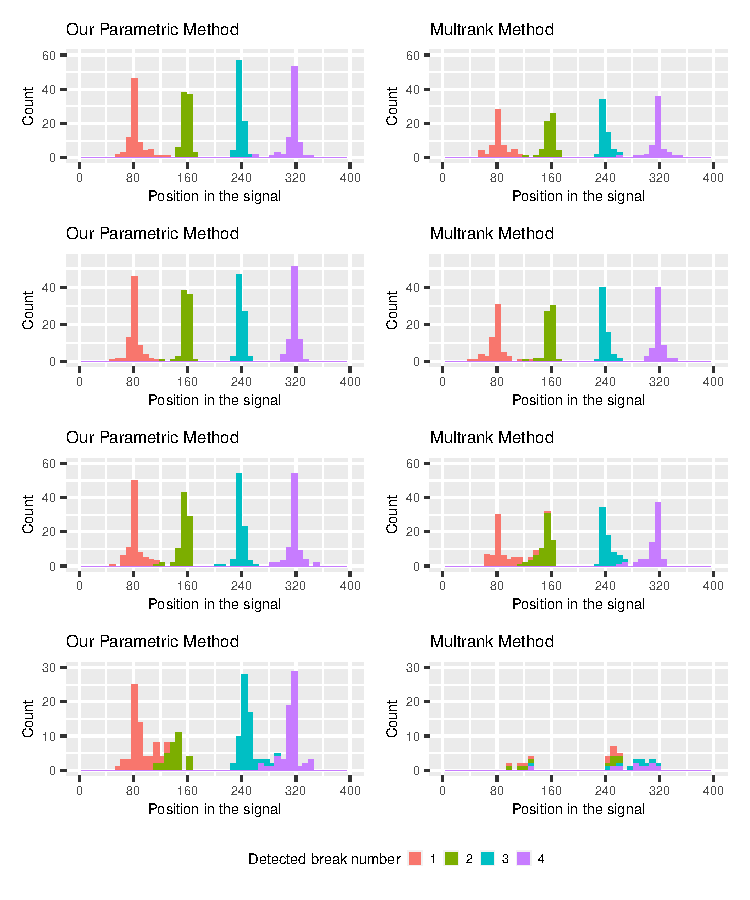
\includegraphics{figs/Chap4/detect_comp.pdf}
    \caption{Precision of the estimated change-points for both methods.}
    \label{fig:prec_sim}
\end{figure}


\subsection{Testing the estimation procedure with an unknown $\sigma$}\label{chp:4:4:3}

We test the procedure developed in Section \ref{chp:4:3:2} on two different simulated signals $\bm y$ and $\bm z$. We set $Q$ as the Weibull distribution with $\lambda$ denoting the scale parameter and $\sigma$ the shape parameter. We suppose that the changes occur in $\lambda$ and that $\sigma$ is fixed throughout the signal. The two simulated signals with their respective parameter information are illustrated in Figures \ref{fig:y_sim1} and \ref{fig:y_sim2}. 

$\bm y$ is $n = 500$ sized signal. The change point are located at position 120, 185, 310, 365. The shape parameter is set to $\sigma = 0.33$. The scale parameters on each segment are $(\lambda^*_k)_{k = 0}^5 = (2,1,3,1,2)$. Every value less than the median of $\bm y$ was censored corresponding to the censoring threshold $a = 0.67$.

$\bm z$ is a $n = 1000$ sized signal. The change point are located at position 120, 185, 310, 365, 495, 580, 700 and 850. The shape parameter is set to $\sigma = 0.33$. The scale parameters on each segment are $(\lambda^*_k)_{k = 0}^8 = (1/50, 1/10, 1/100, 1/5, 1/100, 1/20, 1/70,1, 1/50)$. Every value less than the median of $\bm z$ was censored corresponding to the censoring threshold $a = 0.01$.

\begin{figure}[htbp]
    \centering
    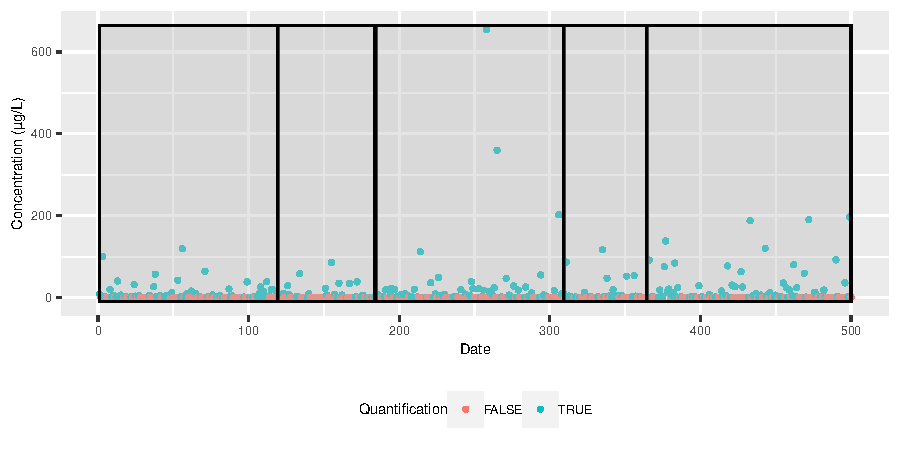
\includegraphics{figs/Chap4/y_sim1.pdf}
    \caption{Simulated signal $\bm y$ of size = $n = 500$. The change point are located at position $120,185,310,365$. The segments are illustrated in black. The shape parameter is set to $\sigma = 0.33$. The scale parameters on each segment are $(\lambda^*_k)_{k = 0}^5 = (2,1,3,1,2)$. Every value less than the median of $\bm y$ was censored corresponding to the censoring threshold $a = 0.67$.}
    \label{fig:y_sim1}
\end{figure}

\begin{figure}[htbp]
    \centering
    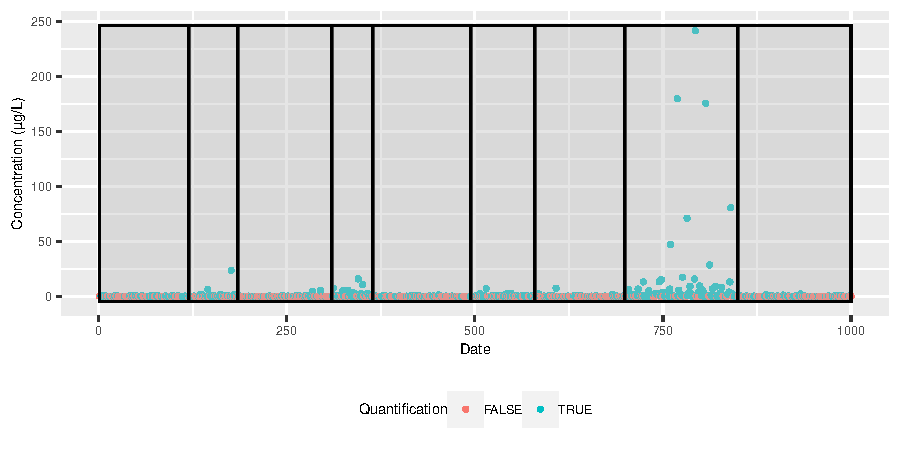
\includegraphics{figs/Chap4/y_sim2.pdf}
    \caption{Simulated signal $\bm z$ of size $n = 1000$. The change point are located at position $ 120, 185, 310, 365, 495, 580, 700, 850 $. The segments are illustrated in black. The shape parameter is set to $\sigma = 0.33$. The scale parameters on each segment are $(\lambda^*_k)_{k = 0}^8 = (1/50, 1/10, 1/100, 1/5, 1/100, 1/20, 1/70,1, 1/50)$. Every value less than the median of $\bm z$ was censored corresponding to the censoring threshold $a = 0.01$.}
    \label{fig:y_sim2}
\end{figure}

Both of outer step strategies presented in Section \ref{chp:4:3:2:2} are implemented to explore the range penalty $[\beta_{min},\beta_{max}]$: 
\begin{itemize}
\item We use a penalty range with 10 evenly spaced values of $\beta$.  
\item We explore the penalty range using CROPS algorithm rules to uncover new values of $\beta$.
\end{itemize}

The values of $\beta_{min}$ and $\beta_{max}$ are set according to the signal lengths. We choose these values so that $\beta_{min}$ corresponds to an overfitting model and $\beta_{max}$ an underfitting one. More precisely, the values are set to $\beta_{min} = \frac{\log(n)}{10}$ and $\beta_{max} = \log(n)$ for $\bm y$; $\beta_{min} = \frac{\log(n)}{4}$ and $\beta_{max} = 2\log(n)$ for $\bm z$.

The results for the penalty values tested for both signals are illustrated in Figures \ref{fig:res_sim_y} and \ref{fig:res_sim_z}.

\begin{figure}[htbp]
    \centering
    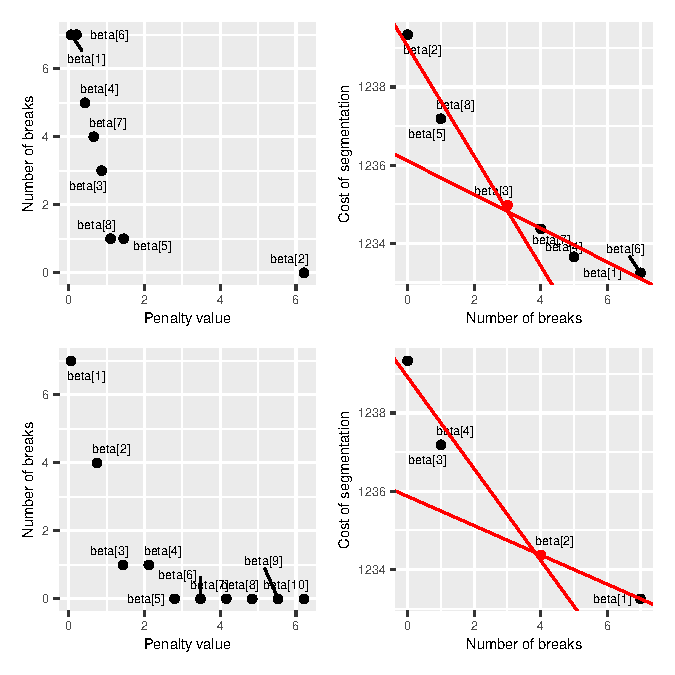
\includegraphics{figs/Chap4/RES_SIM_Y.pdf}
    \caption{Simulation results for signal $\bm y$. \\ 
    Top left figure: plot of the penalty values uncovered by the CROPS procedure. The number of change-points are plotted against their associated penalty values. The annotations give the order in which the penalty were uncovered. \\
    Top right figure: plot of the cost of the resulting segmentations uncovered by the CROPS procedure. The cost of the segmentations are plotted against their associated number of breaks. The red lines represent the two part linear model chosen with the elbow heuristic. The annotations are a reminder of the penalty values in the top left figure to which the segmentations are associated to. \\
    Bottom left figure: plot of the penalty values uncovered using the grid of penalty values. The number of change-points are plotted against their associated penalty values. The annotations give the order in which the penalty were uncovered. \\
    Bottom right figure: plot of the cost of the resulting segmentations uncovered by the penalty grid. The cost of the segmentations are plotted against their associated number of breaks. The red lines represent the two part linear model chosen with the elbow heuristic. The annotations are a reminder of the penalty values in the bottom left figure to which the segmentations are associated to.}
    \label{fig:res_sim_y}
\end{figure}

\begin{figure}[htbp]
    \centering
    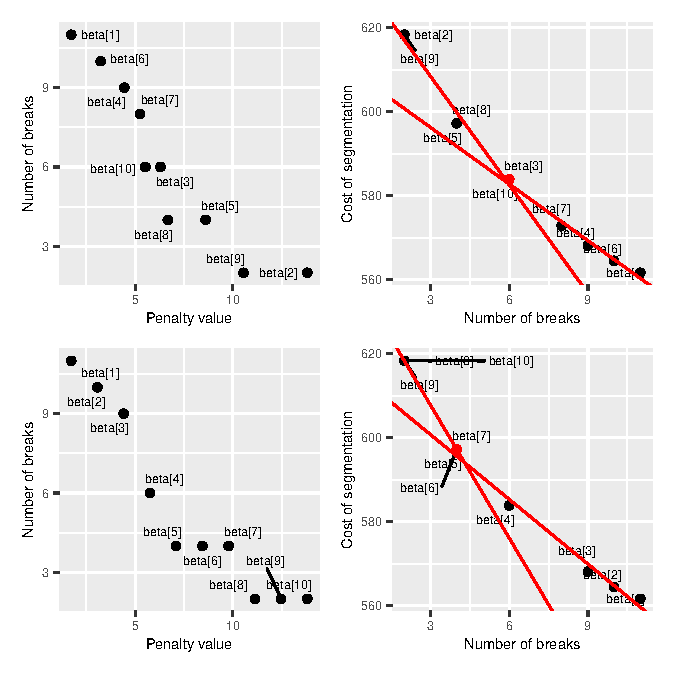
\includegraphics{figs/Chap4/RES_SIM_Z.pdf}
    \caption{Simulation results for signal $\bm z$. \\ 
    Top left figure: plot of the penalty values uncovered by the CROPS procedure. The number of change-points are plotted against their associated penalty values. The annotations give the order in which the penalty were uncovered. \\
    Top right figure: plot of the cost of the resulting segmentations uncovered by the CROPS procedure. The cost of the segmentations are plotted against their associated number of breaks. The red lines represent the two part linear model chosen with the elbow heuristic. The annotations are a reminder of the penalty values in the top left figure to which the segmentations are associated to. \\
    Bottom left figure: plot of the penalty values uncovered using the grid of penalty values. The number of change-points are plotted against their associated penalty values. The annotations give the order in which the penalty were uncovered. \\
    Bottom right figure: plot of the cost of the resulting segmentations uncovered by the penalty grid. The cost of the segmentations are plotted against their associated number of breaks. The red lines represent the two part linear model chosen with the elbow heuristic. The annotations are a reminder of the penalty values in the bottom left figure to which the segmentations are associated to.}
    \label{fig:res_sim_z}
\end{figure}

These results show that:
\begin{itemize}
\item As expected, exploring the penalty range using CROPS is faster than using the penalty grid. Moreover, exploring the penalty range with a regular step can lead to a sub optimal exploration of the penalty values. In Figures \ref{fig:res_sim_z} (top left) and \ref{fig:res_sim_y} (top left), we can see that the estimation procedure was run for several penalty values resulting in the same segmentation. CROPS uncovers segmentation results that can be missed with a regular grid.%more new 
\item When the correct model is present among the uncovered segmentations, the associated estimated parameters are accurate (change point locations, segment parameters and common shape parameter). We can conclude that the estimation procedure is correct provided the correct model is selected (see Figures \ref{fig:detect_sim_y} and \ref{fig:detect_sim_z}). The estimated values of $\sigma$ remain close to its true value even when the incorrect number of change-point is selected. Using the results of the CROPS procedure, the estimated $\sigma$ ranged between $0.334$ and $0.342$ for signal $\bm y$; they ranged between $0.308$ and $ 0.348$ for $\bm z$. 
%The parameter estimation is accurate when the correct number of change-points is present among the uncovered segmentations. 

\item The selection of the segmentation model is made with the elbow heuristic (Figures \ref{fig:res_sim_y} top and bottom right and \ref{fig:res_sim_z} top and bottom right). We can see that it did not select the correct model except when using the penalty grid for signal $\bm y$. We can argue that the correct model was selected by chance in this case because of the step used in the grid. Since we missed some segmentation results, the elbow was more apparent. However, we can see that the elbow method selected a model that was very far from the true setting using the grid in the case of $\bm z$. The model selected with the CROPS results missed some change points both in $\bm y$ and $\bm z$. The change points in positions 467 and 580 were not detected in $\bm z$. The change point in position 133 was not detected for $\bm y$. The $\lambda$ parameters surrounding these change-points in each signal have very close values which can explain the fact they were not detected.     
\end{itemize}

We can conclude that the estimation procedure is working accurately on simulated data. However, the model selection is a complex task only partially fulfilled by the elbow heuristic. Note that other heuristics can be used to select the optimal model. 

In practice, this is not a major issue since we aim at providing several models to the experts. We use the estimation procedure described in Section \ref{chp:4:3} in the subsequent chapter on a real concentration data. For presentation purposes, we will use the elbow heuristic to select a segmentation on these data as well but we keep in mind that the resulting segmentation may not be the optimal one and that neighbouring segmentation should be also explored. In Chapter \ref{chp:6}, we overcome this selection problem by presenting all segmentation models found in an interactive application. 


\begin{figure}[htbp]
    \centering
    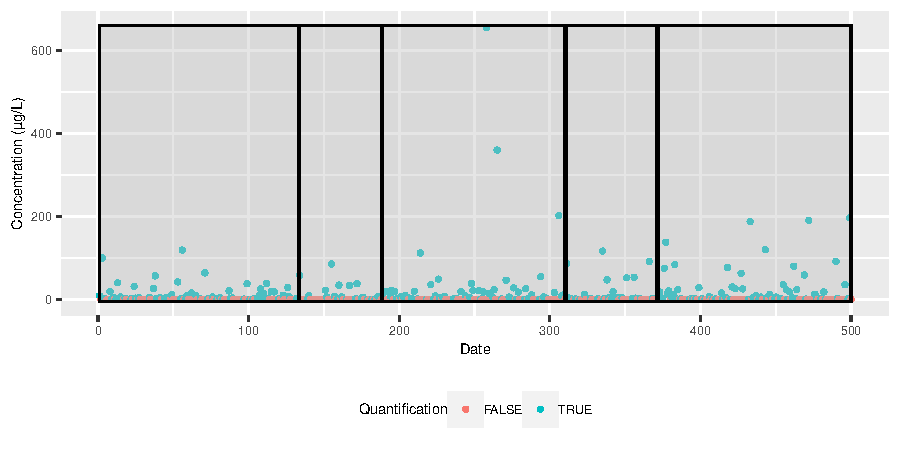
\includegraphics{figs/Chap4/y_sim_detect.pdf}
    \caption{Segmentation results with correct number of change-points for signal $\bm y$. The estimated change-points are located at positions $133,188,310,371$. The (approximated) estimated scale parameter values are $(\widehat{\lambda}_k)_{k=0}^4 = (1.62,1.05,2.69,1.49,2.99)$. The estimated shape parameter value is $\widehat{\sigma} = 0.34$.}
    \label{fig:detect_sim_y}
\end{figure}

\begin{figure}[htbp]
    \centering
    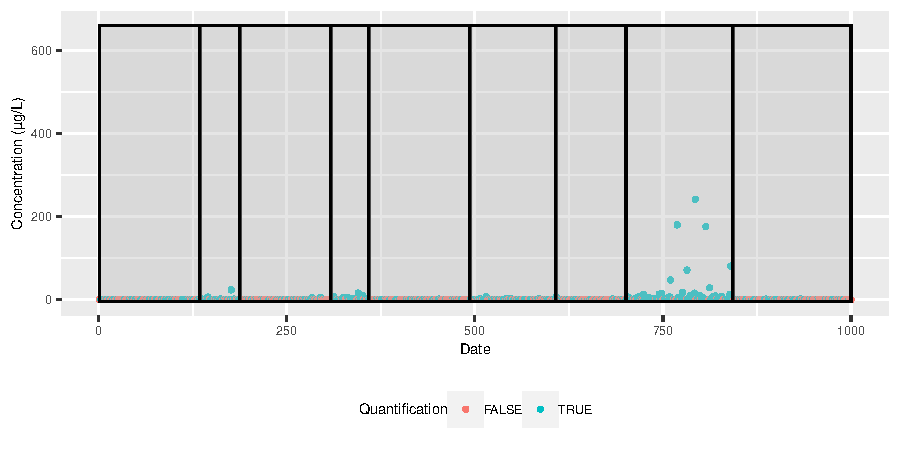
\includegraphics{figs/Chap4/y_sim2_detect.pdf}
    \caption{Segmentation results with correct number of change-points for signal $\bm z$. The estimated change-points are located at positions $134,187,308,359,493,607,701,842$. The (approximated) estimated scale parameter values are $(\widehat{\lambda}_k)_{k=0}^8 = (\frac{1}{55},\frac{1}{10},\frac{1}{78},\frac{1}{4},\frac{1}{92},\frac{1}{19},\frac{1}{74},1,\frac{1}{56})$. The estimated shape parameter value is $\widehat{\sigma} = 0.34$.}
    \label{fig:detect_sim_z}
\end{figure}


\clearpage

\section{Chapter summary}

This Chapter designs and tests an adapted change-point detection method for concentration data. The censoring is handled by the cost function choice in Section \ref{chp:4:2}. More precisely, using a parametric approach as presented in Chapter \ref{chp:3}, the likelihood is adapted to distinguish cases were a measure is censored or not. The censoring becomes critical for computing the maximum likelihood estimate of a segment when all observations are censored. This could cause issues in the identifiability of segments parameters which would compromise the detection method capacity. One way to circumvent this problem is to introduce a new regularization parameter in the detection that is a maximum value for the parameter value. The estimation strategy is also discussed in this Section \ref{chp:4:3}. An estimation scheme where some dimensions of the parameter vector are fixed in time and other can vary across segments is devised. Experiments of Section \ref{chp:4:4} ensure that, if enough data is available to evaluate a segment, the parametric method performs decently and can outclass a non parametric method that can also take censored data into account. 

Chapter \ref{chp:5} combines the results of temporal change-point detection using the parametric method developed in this Chapter with statistical methods to deal with the spatial heterogeneity. The obtention of homogeneous temporal sub signal in the concentrations values provides the temporal context in which the spatial analysis is conducted. In particular, in this homogeneous temporal setting, it is interesting to look for geographical areas that had concentration values that differ from others. Constructing these areas and comparing them is the main topic of Chapter \ref{chp:5}. Chapter \ref{chp:6} is the presentation of the results of Chapter \ref{chp:5} and \ref{chp:4} applied to the concentration data of substance. The results of all methods are all gathered using an interactive presentation tool.     

       

 